\chapter{Architettura del Sistema Proposto}
\label{chap:architettura}

\section{Obiettivi e funzionalità del sistema}
Il sistema proposto è stato progettato per affrontare direttamente le limitazioni per l'adozione diffusa del 3D Gaussian Splatting identificate nel capitolo precedente, trasformando una tecnologia prevalentemente accademica in una soluzione accessibile e user-friendly.

\subsection{Obiettivi di progetto}

\paragraph{Migliore accesso alla tecnologia}
L'obiettivo primario consiste nel rendere il 3D Gaussian Splatting accessibile a utenti senza competenze tecniche specialistiche in computer graphics o machine learning. Il sistema deve eliminare le barriere di ingresso tipiche degli strumenti di ricerca, permettendo a professionisti di settori diversi - dal design alla produzione multimediale - di sfruttare le potenzialità della tecnologia attraverso un'interfaccia intuitiva.

\paragraph{Unificazione di strumenti frammentati}
Il secondo obiettivo riguarda l'integrazione di funzionalità attualmente disperse in implementazioni separate. Il sistema deve fornire una piattaforma unificata che comprenda training, visualizzazione e gestione modelli, eliminando la necessità di utilizzare tool specifici incompatibili tra loro e riducendo significativamente la curva di apprendimento.

\paragraph{Automazione del workflow tecnico}
Il terzo obiettivo è l'automazione dell'intero processo, dalla preparazione dei dati alla visualizzazione finale, riducendo al minimo l'intervento manuale e la possibilità di errori. Questo include la gestione automatica di preprocessing, configurazione parametri e troubleshooting di problemi comuni.

\subsection{Funzionalità del sistema}
Per raggiungere questi obiettivi, il sistema implementa le seguenti funzionalità core:

\paragraph{Interfaccia web guidata}
Il sistema fornisce un'interfaccia web responsive che guida l'utente attraverso un processo step-by-step, dalla selezione del video di input alla visualizzazione del modello 3D finale. L'interfaccia integra:

\begin{itemize}
\item \textbf{Processo guidato}: Workflow sequenziale con istruzioni chiare per ogni fase
\item \textbf{Validazione intelligente}: Controllo automatico della qualità e formato dei file di input
\item \textbf{Feedback}: Indicatore della fase in cui si trovano le elaborazioni
\item \textbf{Documentazione contestuale}: Spiegazioni integrate e suggerimenti per ottimizzare i risultati
\end{itemize}

\paragraph{Training multi-algoritmo integrato}
La piattaforma integra tre diversi approcci di training del Gaussian Splatting in un'unica interfaccia:

\begin{itemize}
\item \textbf{Standard 3DGS}: Implementazione baseline per risultati di alta qualità
\item \textbf{MCMC Gaussian Splatting}: Approccio probabilistico per miglioramento della qualità e riduzione artefatti
\item \textbf{Taming 3DGS}: Ottimizzazione per risorse computazionali limitate
\end{itemize}

L'utente può selezionare l'algoritmo desiderato attraverso un'interfaccia semplificata con parametri preconfigurati per casi d'uso comuni.

\paragraph{Pipeline di processing automatizzata}
Il sistema implementa una pipeline completamente automatizzata che gestisce:

\begin{enumerate}
\item \textbf{Preprocessing video}: Estrazione automatica di frame ottimali dal video di input
\item \textbf{Structure from Motion}: Generazione automatica della point cloud iniziale
\item \textbf{Training asincrono}: Elaborazione in background con notifiche di completamento
\item \textbf{Upload modello}: Upload su repository del modello 3D generato dal training
\item \textbf{Post-processing}: Generazione e salvataggio delle metriche di elaborazione
\end{enumerate}

\begin{figure}[htbp]
	\centering
	\adjustbox{width=0.8\textwidth,center,keepaspectratio}{
		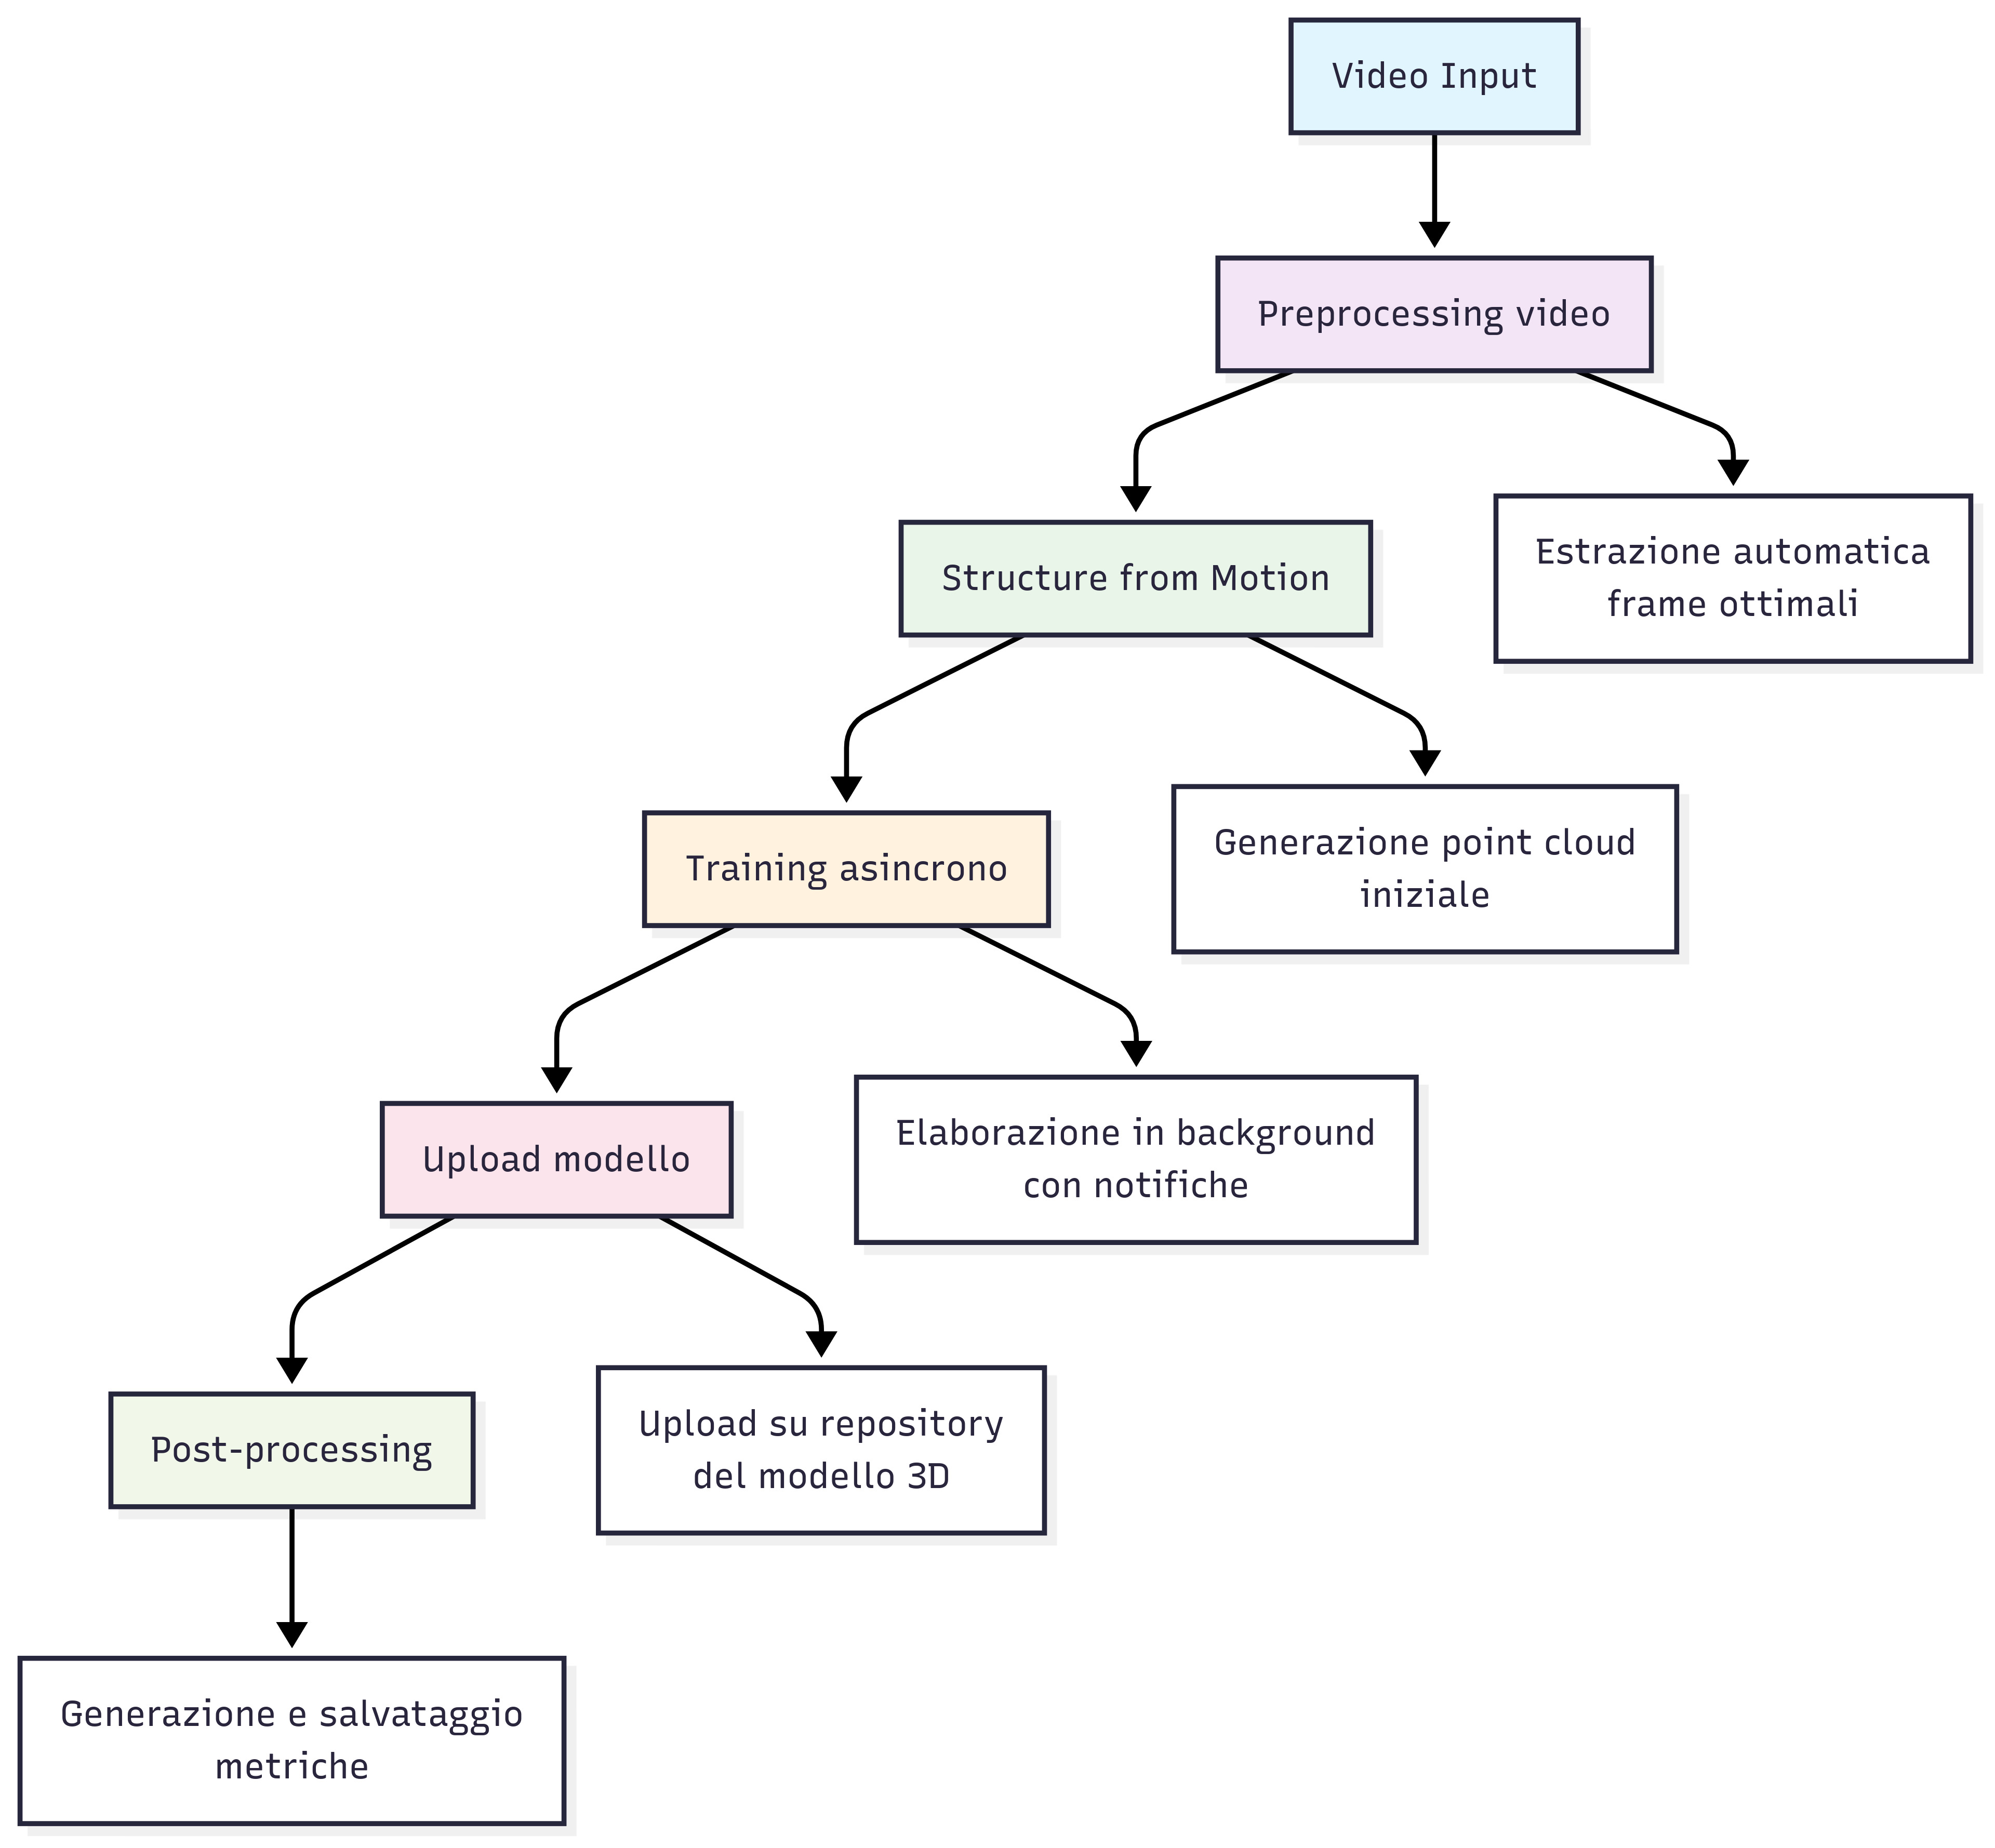
\includegraphics{images/functional_workflow.jpg}
	}
	\caption{Pipeline di processing automatizzata}
	\label{fig:functional_workflow}
\end{figure}

\paragraph{Visualizzazione 3D integrata}
La piattaforma include un viewer 3D web-based che permette:

\begin{itemize}
\item \textbf{Rendering real-time}: Visualizzazione immediata dei modelli generati
\item \textbf{Controlli interattivi}: Navigazione 3D intuitiva con mouse/touch
\item \textbf{Valutazione}: Visualizzazione delle statistiche come FPS e numero di gaussiane generate
\end{itemize}

\paragraph{Gestione trasparente delle risorse}
Il sistema nasconde la complessità tecnica attraverso:

\begin{itemize}
\item \textbf{Containerizzazione}: Ambiente di esecuzione isolato e riproducibile
\item \textbf{Gestione automatica GPU}: Allocazione ottimale delle risorse computazionali
\item \textbf{Scaling adattivo}: Gestione automatica del carico di lavoro
\item \textbf{Monitoring integrato}: Raccolta automatica di metriche di performance e qualità
\end{itemize}

\subsection{Benefici attesi}

L'implementazione di queste funzionalità mira a produrre i seguenti benefici:
\begin{itemize}
    \item \textbf{Riduzione time-to-market}: Dalla creazione del contenuto alla visualizzazione 3D in minuti invece che ore o giorni richiesti da workflow tradizionali.
    \item \textbf{Accessibilità ampliata}: Estensione dell'utilizzo del 3D Gaussian Splatting a settori non tecnici come marketing, e-commerce, architettura e produzione di contenuti.
    \item \textbf{Standardizzazione del processo}: Etablishment di best practices e workflow standardizzati per la creazione di contenuti 3D da video.
    \item \textbf{Riduzione costi}: Eliminazione della necessità di competenze specialistiche dedicate e riduzione dei tempi di training del personale.
\end{itemize}

\section{Organizzazione a Layer}

Il sistema proposto implementa un'architettura distribuita a microservizi progettata per gestire l'intero workflow del 3D Gaussian Splatting, dall'upload del contenuto video alla visualizzazione dei modelli 3D generati. La Figura \ref{fig:system_architecture} presenta una vista complessiva dell'architettura, evidenziando i componenti principali e i loro pattern di interazione.
L'architettura è strutturata in layer distinti, ciascuno con responsabilità specifiche e interfacce ben definite, seguendo i principi di separazione delle responsabilità e scalabilità indipendente. Questa organizzazione logica non implica una separazione fisica rigida, ma piuttosto una strutturazione delle responsabilità che può essere implementata all'interno di uno o più servizi containerizzati.

\begin{figure}[htbp]
	\centering
	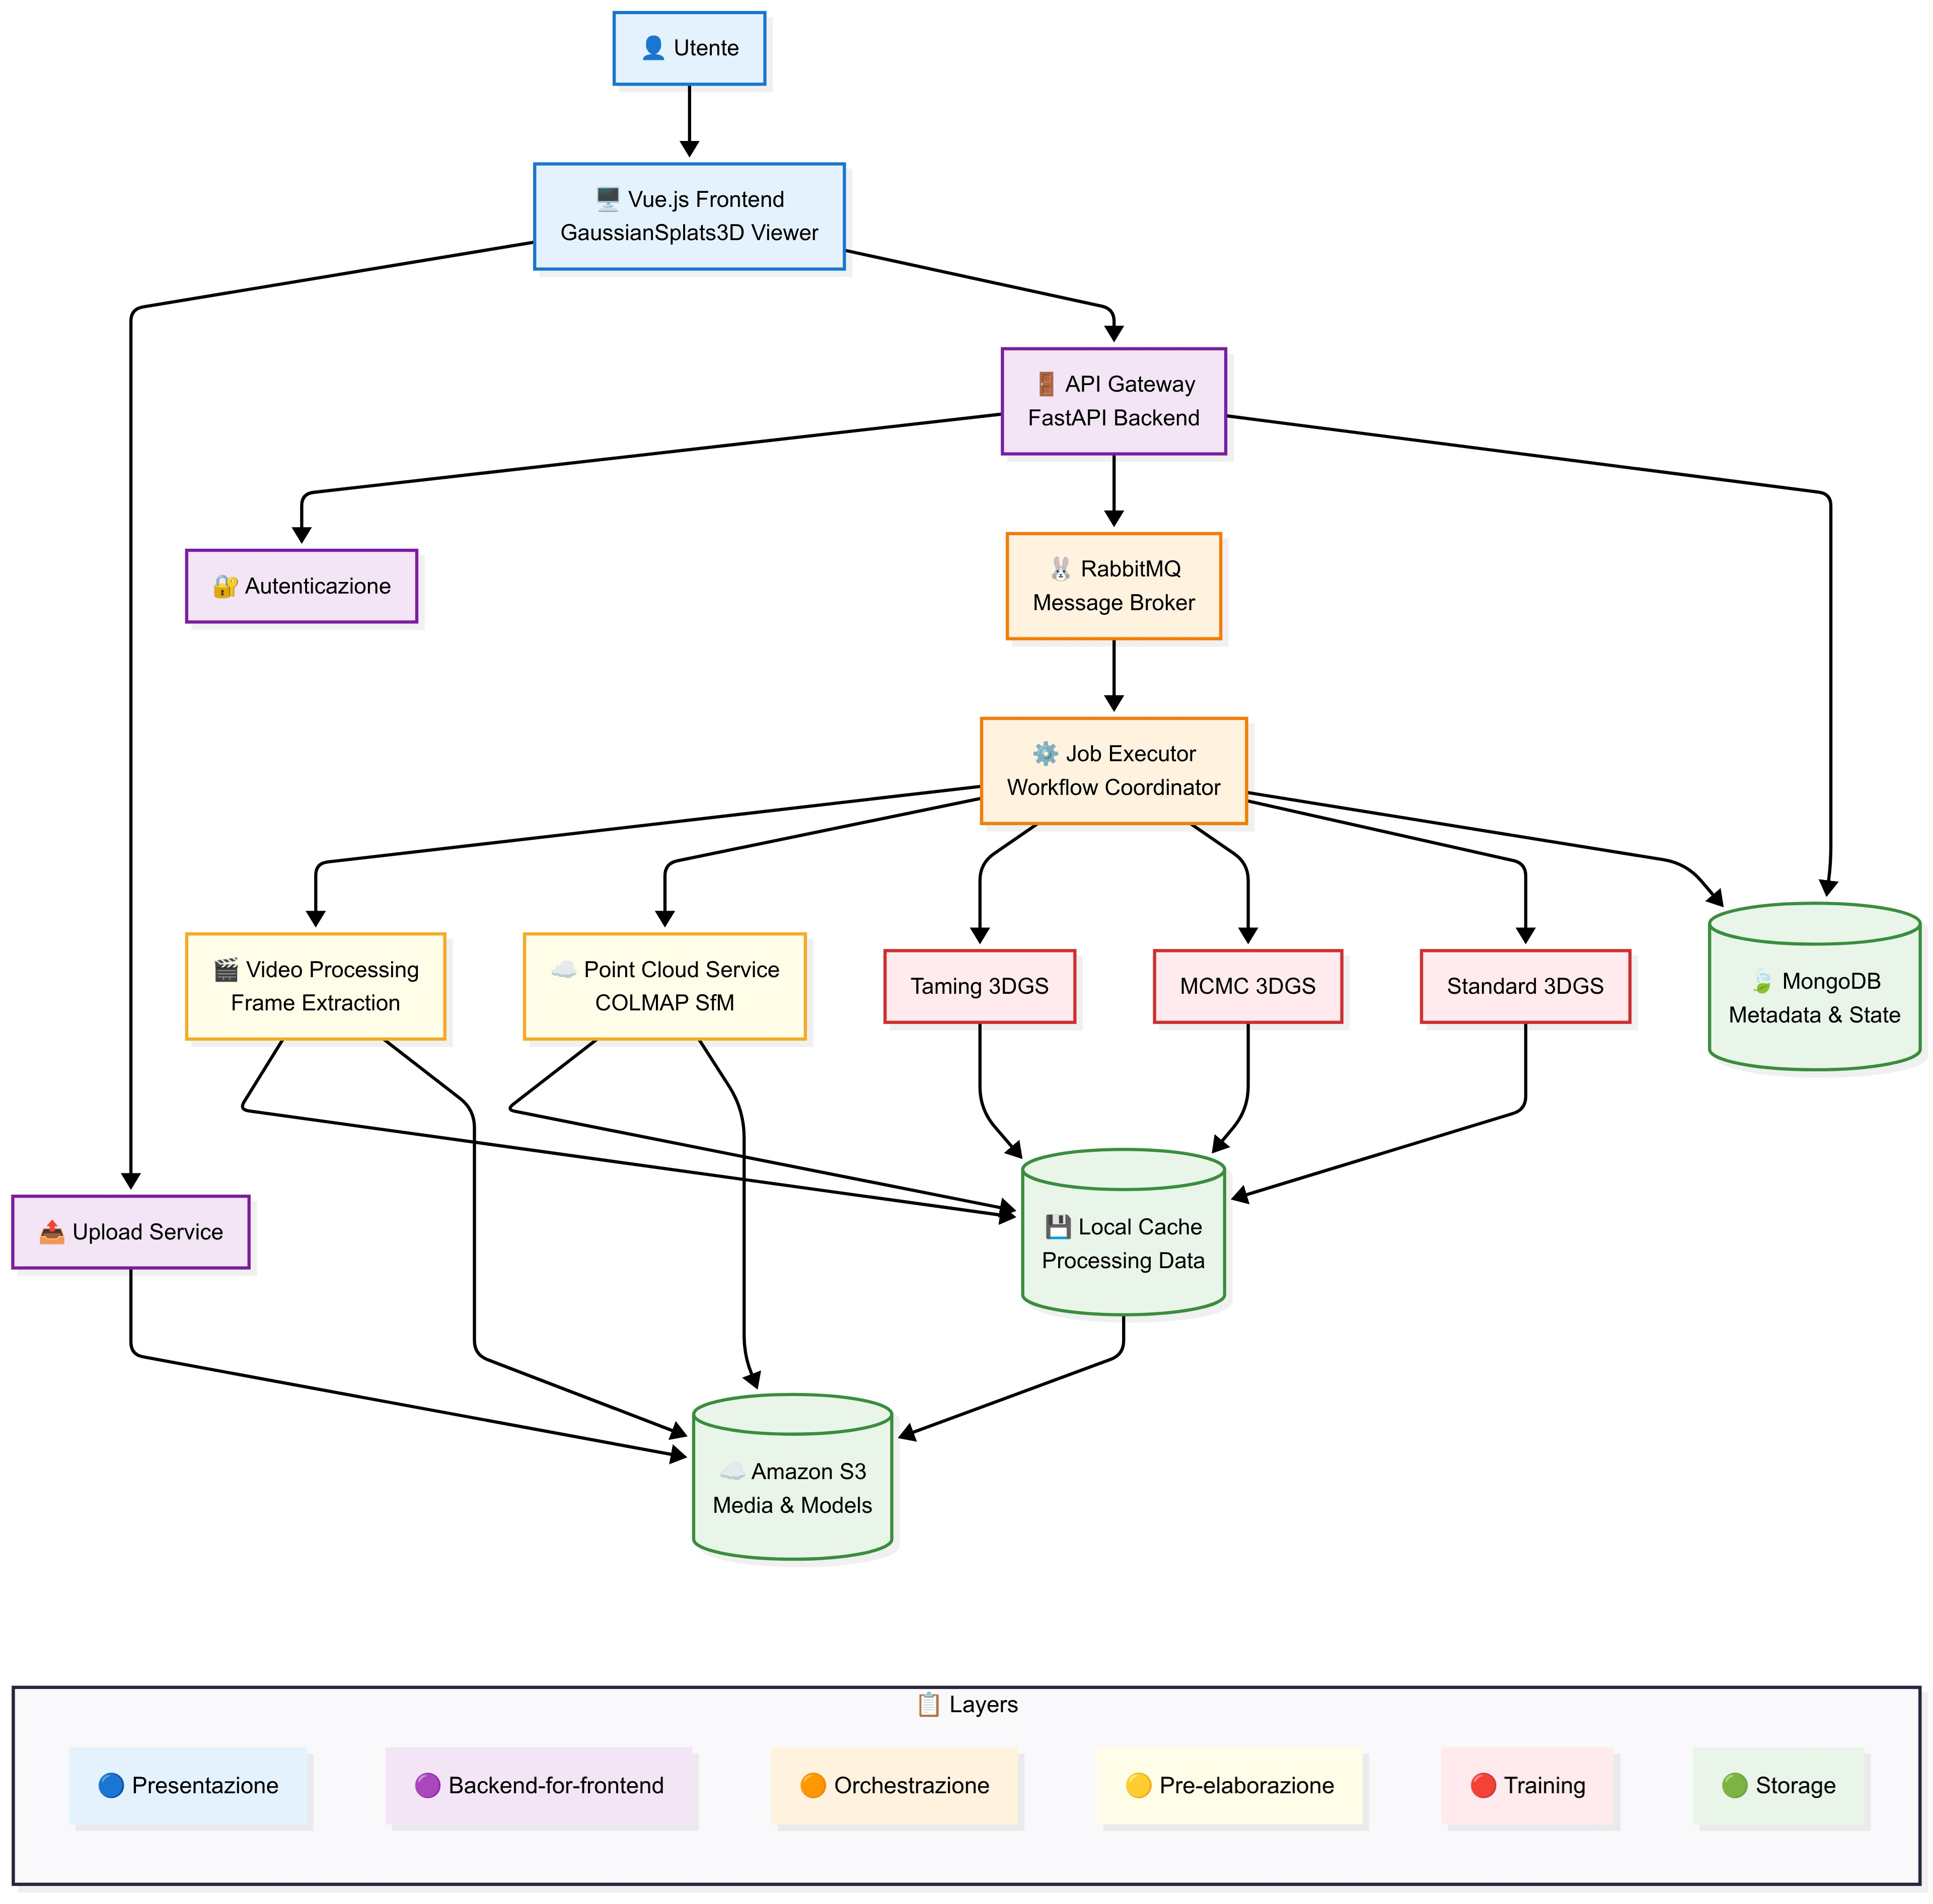
\includegraphics[width=\textwidth]{images/diagramma_architettura.jpg}
	\caption{Architettura complessiva del sistema distribuito}
	\label{fig:system_architecture}
\end{figure}


\subsection{Layer di Storage}

Il \textbf{layer di storage} implementa una strategia ibrida che combina MongoDB per metadati e stato delle elaborazioni, Amazon S3 per contenuti multimediali e modelli 3D che si appoggia a sua volta ad una cache locale per dati di processing temporanei.

\subsection{Layer di Orchestrazione}

Il \textbf{layer di orchestrazione} rappresenta il cuore coordinativo del sistema, implementato attraverso RabbitMQ come message broker e il Job Executor come coordinatore del workflow. Questo layer gestisce la comunicazione asincrona tra i componenti e implementa un pattern Producer-Consumer ibrido che garantisce l'esecuzione sequenziale delle fasi di elaborazione. La scelta di RabbitMQ assicura persistenza dei messaggi, gestione delle code specializzate e resilienza in caso di fallimenti temporanei.

\subsection{Layer di Pre-elaborazione}
Il \textbf{layer di preprocessing} comprende i servizi specializzati responsabili dell'elaborazione preliminare dei dati: Video Processing per l'estrazione dei frame dal video di input e Point Cloud Service per la ricostruzione geometrica tramite COLMAP SfM.

\subsection{Layer di Training}
Il \textbf{layer di training} include i Training Services che eseguono gli algoritmi di Gaussian Splatting nelle diverse implementazioni (Taming 3DGS, MCMC 3DGS e Standard 3DGS), utilizzando le risorse computazionali GPU per l'addestramento dei modelli.

\subsection{Layer Backend-for-Frontend}
Il \textbf{layer Backend-for-Frontend} funge da punto di ingresso unificato per tutte le richieste del sistema, implementando pattern di routing, autenticazione e gestione delle richieste. Questo layer è univocamente rappresentato dall'applicazione (e container) API Gateway, è sviluppata in FastAPI ed espone endpoint REST standardizzati permettendo l'accesso ai servizi sottostanti.

\subsection{Layer di Presentazione}
Il \textbf{layer di presentazione} costituisce l'interfaccia utente del sistema e comprende l'applicazione web sviluppata in Vue.js integrata con il viewer GaussianSplats3D. Questo layer gestisce l'interazione utente, la visualizzazione dei modelli generati e la gestione degli stati dell'interfaccia. La scelta di Vue.js consente un'architettura component-based leggera che facilita la manutenibilità e l'estensibilità dell'interfaccia.

\section{Principi e pattern architetturali}

\subsection{Principi di design}
L'architettura del sistema è stata progettata rispondendo alle sfide specifiche del 3D Gaussian Splatting come tecnologia emergente. A differenza delle applicazioni web tradizionali, il Gaussian Splatting presenta caratteristiche uniche che richiedono decisioni architetturali mirate: elaborazioni GPU-intensive con tempi variabili da minuti a ore, algoritmi in rapida evoluzione, gestione di contenuti multimediali di grandi dimensioni e necessità di isolamento per operazioni hardware-critical.

I principi di design adottati mirano a trasformare una tecnologia di ricerca complessa in una piattaforma accessibile e robusta. L'approccio privilegia la separazione delle preoccupazioni per isolare la complessità computazionale dalle interfacce utente, la scalabilità selettiva per ottimizzare l'uso di risorse costose, e la modularità per facilitare l'integrazione di nuovi algoritmi e l'evoluzione del sistema nel tempo.

Questi principi si concretizzano in scelte implementative specifiche che bilancino semplicità d'uso, efficienza operativa e flessibilità tecnica.

\subsubsection{Separazione delle responsabilità per processing intensivo}
Sebbene un'architettura monolitica possa gestire processing asincrono 
attraverso threading, l'approccio a microservizi offre vantaggi specifici 
per il Gaussian Splatting: isolamento degli errori hardware-intensive, 
scalabilità selettiva delle risorse GPU, e deployment indipendente di 
algoritmi in evoluzione.
L'approccio a microservizi permette di separare logicamente:

\begin{itemize}
    \item \textbf{Servizi di interfaccia}: Frontend e API che rimangono sempre responsivi
    \item \textbf{Servizi di processing}: Dedicati esclusivamente al training intensivo
    \item \textbf{Servizi di supporto}: Gestione dati, code messaggi e storage
\end{itemize}


Queste funzionalità si traducono in un'architettura tecnica specifica che verrà dettagliata nelle sezioni successive, dimostrando come gli obiettivi di alto livello si concretizzino in scelte implementative precise.

\begin{figure}[htbp]
	\centering
	\adjustbox{width=0.9\textwidth,center,keepaspectratio}{
		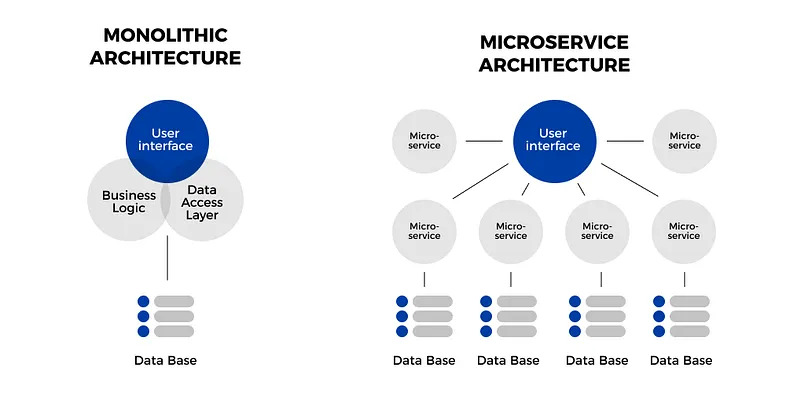
\includegraphics{images/monolith_vs_microservices.jpg}
	}
	\caption{Architettura monolita vs architettura a microservizi}
	\label{fig:monolith_vs_microservices}
\end{figure}

\subsubsection{Scalabilità orizzontale specializzata}
La natura del training di Gaussian Splatting, che richiede hardware dedicato (GPU), rende particolarmente vantaggiosa la possibilità di scalare orizzontalmente solo i componenti computazionalmente intensivi. I servizi di training, essendo containerizzati e stateless, possono essere deployati su multiple macchine dotate di GPU specializzate, mentre frontend e API rimangono centralizzati su hardware meno specializzato.
Questa separazione consente di:

\begin{itemize}
    \item \textbf{Ottimizzare i costi}: hardware GPU costoso utilizzato solo per training e il preprocessing
    \item \textbf{Gestire il carico}: aAggiungere capacità computazionale senza modificare altri servizi
    \item \textbf{Isolamento degli errori}: crash o indisponibilità del training non compromette l'interfaccia utente
\end{itemize}

\subsubsection{Deployment e manutenzione indipendente}
L'architettura modulare facilita lo sviluppo e la manutenzione del sistema, permettendo di aggiornare, testare e deployare ogni componente indipendentemente. Questo è particolarmente vantaggioso per un progetto che integra algoritmi di training in evoluzione (Standard, MCMC, Taming), dove ogni implementazione può essere aggiornata senza impattare gli altri moduli.

\begin{figure}[htbp]
	\centering
	\adjustbox{width=0.9\textwidth,center,keepaspectratio}{
		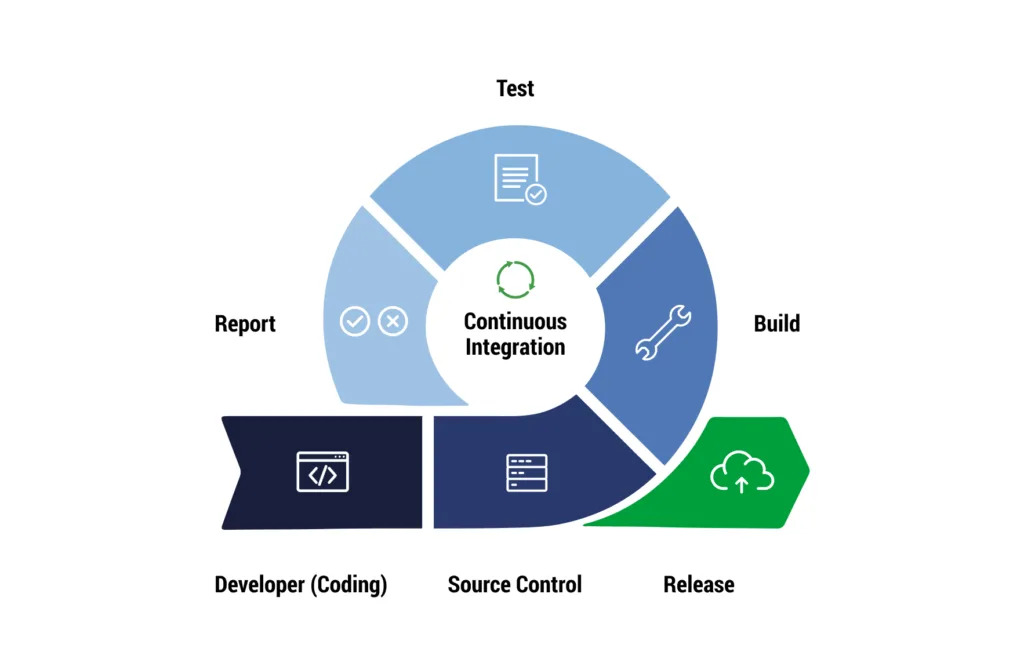
\includegraphics{images/continuous_integration.jpg}
	}
	\caption{Schema della continuous integration}
	\label{fig:continuous_integration}
\end{figure}

\subsection{Pattern architetturali implementati}

Per realizzare i principi di design descritti, il sistema adotta pattern architetturali consolidati, adattati alle specifiche esigenze del 3D Gaussian Splatting. Questi pattern forniscono soluzioni concrete per gestire la complessità del workflow, garantire la resilienza del sistema e ottimizzare l'uso delle risorse computazionali.

I pattern selezionati operano sinergicamente per creare un'architettura che supporta elaborazioni asincrone lunghe, gestione robusta degli errori e scalabilità delle operazioni intensive.

\subsubsection{Architettura Event-driven}
Il sistema implementa un'architettura guidata dagli eventi attraverso una coda di messaggi che coordina l'esecuzione delle diverse fasi di processing. Ogni completamento di fase genera un evento che triggera la fase successiva, creando un workflow asincrono e resiliente.\newline\newline
\textbf{Vantaggi per il Gaussian Splatting}:
\begin{itemize}
	\item \textbf{Gestione della coda}: Serializzazione automatica dei job per gestire la limitazione di GPU singola
	\item \textbf{Retry automatico}: Eventi possono essere riaccodati in caso di fallimento
	\item \textbf{Monitoring}: Stato del workflow tracciabile attraverso gli eventi
\end{itemize}

\begin{figure}[htbp]
	\centering
	\adjustbox{width=0.9\textwidth,center,keepaspectratio}{
		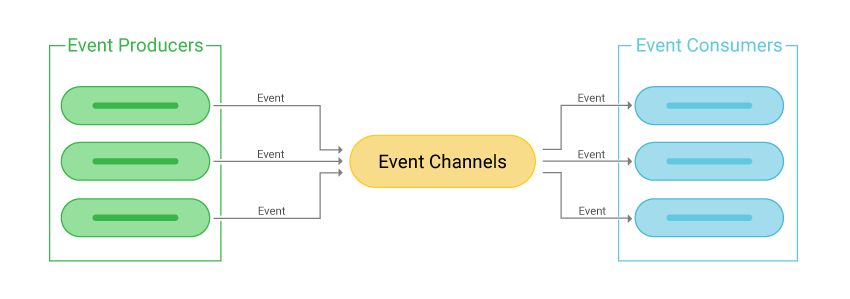
\includegraphics{images/event_driven_architecture.jpg}
	}
	\caption{Architettura Event-driven}
	\label{fig:event_driven_architecture}
\end{figure}

\subsubsection{Pipeline Pattern}
Il processing del Gaussian Splatting segue naturalmente un pattern pipeline con handoff espliciti tra fasi:

\begin{itemize}
	\item \textbf{Estrazione frame} → Output: frame video + metadati
	\item \textbf{Structure from Motion} → Output: point cloud + pose camere
	\item \textbf{Training} → Output: modello 3D ottimizzato
\end{itemize}

Ogni fase produce output standardizzati che vengono consumati dalla fase successiva, permettendo parallelizzazione e reprocessing selettivo.

\subsubsection{Caching e Storage Pattern}

Il sistema adotta una strategia di gestione dati multi-livello che combina diversi pattern architetturali per ottimizzare prestazioni, resilienza e ciclo di vita dei contenuti multimediali. L'approccio integra tre pattern complementari specificamente adattati alle caratteristiche del 3D Gaussian Splatting.

\paragraph{Cache-Aside Pattern per performance}
Il sistema implementa una strategia di caching a due livelli per ridurre latenza e costi di accesso ai dati:

\begin{algorithm}[h]
	\caption{Cache-Aside Pattern per gestione risorse}
	\SetAlgoLined
	\KwIn{resource\_identifier}
	\KwOut{resource\_data}
	
	\eIf{resource exists in local\_cache}{
		\Return{load\_from\_local\_cache(resource\_identifier)}\;
	}{
		resource\_data $\leftarrow$ fetch\_from\_remote\_storage(resource\_identifier)\;
		save\_to\_local\_cache(resource\_identifier, resource\_data)\;
		\Return{resource\_data}\;
	}
\end{algorithm}

Questo approccio è particolarmente efficace per file di grandi dimensioni tipici del Gaussian Splatting, riducendo significativamente i costi e i tempi di accesso a S3 durante le operazioni intensive.

\paragraph{Staging Pattern per persistenza intermedia}
Amazon S3 funge da storage intermedio tra le fasi del workflow, implementando un pattern staging che garantisce:

\begin{itemize}
	\item \textbf{Persistenza}: Risultati intermedi sopravvivono a restart dei servizi
	\item \textbf{Reprocessing selettivo}: Possibilità di ripartire da fasi specifiche già completate
	\item \textbf{Auditability}: Tracciabilità completa dei dati prodotti durante l'elaborazione
\end{itemize}

\paragraph{Hybrid Storage per ciclo di vita dati}
La strategia combina diversi livelli di storage ottimizzati per i pattern di accesso specifici del Gaussian Splatting:

\begin{itemize}
	\item \textbf{Storage locale}: Cache temporanea per elaborazioni attive con accesso veloce, riduzione latenza I/O e cleanup automatico
	\item \textbf{Amazon S3 Standard}: Repository persistente per video originali e modelli finali con durabilità, scalabilità e versioning
	\item \textbf{Processing cache}: Dati intermedi (frame, point clouds) mantenuti localmente per supportare reprocessing parziale
\end{itemize}

L'architettura mantiene tutti i dati persistenti per massimizzare la flessibilità operativa, privilegiando la funzionalità di reprocessing e la semplicità gestionale. Questo approccio conservativo garantisce la stabilità del workflow, elemento centrale per l'esperienza utente del sistema.
\newpage
\section{Containerizzazione con Docker e Docker Compose}
\subsection{Isolamento delle dipendenze specializzate}
Ogni algoritmo di training del Gaussian Splatting presenta dipendenze specifiche e spesso conflittuali:

\begin{itemize}
    \item \textbf{Versioni CUDA}: Diverse implementazioni richiedono versioni specifiche di CUDA (driver NVIDIA)
    \item \textbf{Librerie Python}: Conflitti tra versioni di PyTorch, NumPy e librerie di computer vision
    \item \textbf{Configurazioni hardware}: Ottimizzazioni specifiche per GPU diverse
\end{itemize}

\subsection{Orchestrazione con Docker Compose}
Docker Compose facilita la gestione dell'intero stack applicativo, definendo in modo dichiarativo:

\begin{itemize}
    \item \textbf{Networking}: Comunicazione sicura tra container
    \item \textbf{Volume mounting}: Condivisione dati tra servizi
    \item \textbf{Environment variables}: Configurazione centralizzata
    \item \textbf{Service dependencies}: Ordine di avvio dei servizi
\end{itemize}

Sebbene il deployment attuale avvenga su singola macchina per ragioni di sviluppo, l'architettura containerizzata prepara il sistema per un futuro deployment distribuito su cluster.

\subsection{Gestione risorse GPU}
La containerizzazione permette di gestire in modo granulare l'accesso alle risorse GPU, garantendo che il container di training abbia accesso esclusivo alle GPU disponibili, evitando conflitti di risorse e ottimizzando le performance.

\begin{figure}[htbp]
	\centering
	\adjustbox{width=0.9\textwidth,center,keepaspectratio}{
		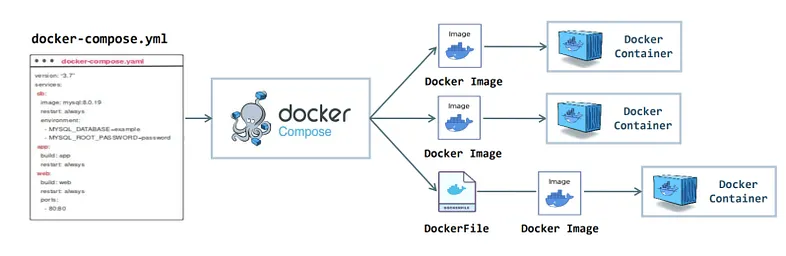
\includegraphics{images/docker_compose.jpg}
	}
	\caption{Architettura con Docker Compose}
	\label{fig:docker_compose}
\end{figure}

\newpage

\section{Gestione asincrona e code messaggi}
Il sistema adotta un'architettura di messaggistica progettata per l'efficienza e la robustezza. La strategia centrale consiste nel separare completamente i dati dai messaggi di controllo: le code contengono esclusivamente identificativi dei modelli, mentre MongoDB centralizza tutti i parametri e lo stato di esecuzione.

\subsection{Code leggere per workflow complessi}
Ogni fase del pipeline (estrazione, SfM, training) utilizza una coda dedicata che trasporta solo gli ID dei modelli da processare. Questa scelta elimina la duplicazione di dati nelle code e mantiene i messaggi estremamente compatti, migliorando le prestazioni del sistema di messaggistica anche con carichi intensivi.

\subsection{Stato sempre sincronizzato}
All'avvio di ogni fase, il servizio responsabile interroga MongoDB per recuperare configurazione, stato precedente e metadati aggiornati. Questo pattern garantisce che ogni elaborazione operi sempre sui dati più recenti, eliminando inconsistenze dovute a messaggi obsoleti o duplicati.

\subsection{Resilienza e reprocessing selettivo}
I fallimenti vengono gestiti con arresti controllati che preservano lo stato raggiunto, consentendo analisi dettagliate e retry mirati. Il sistema supporta riprocessing selettivo: un modello può essere rigenerato partendo da qualsiasi fase già completata, evitando elaborazioni ridondanti e ottimizzando l'utilizzo delle risorse GPU.

Questo design bilancia efficienza computazionale e flessibilità operativa, requisiti essenziali per un sistema di produzione dedicato al 3D Gaussian Splatting.

\section{Flusso di elaborazione end-to-end}
Il flusso di elaborazione del sistema segue un approccio sequenziale orchestrato attraverso code di messaggi specializzate. Ogni fase del workflow è gestita da job specifici che, una volta completati, innescano automaticamente la fase successiva della pipeline.
\subsection{Fase di Upload e Inizializzazione}
Il processo inizia con l'upload del video da parte dell'utente attraverso il frontend. Il sistema implementa un meccanismo di upload sicuro basato su presigned URL: il frontend richiede al backend un URL temporaneo per il caricamento diretto sull'object storage, evitando il transito del contenuto multimediale attraverso il backend API. Completato l'upload, il frontend effettua una richiesta POST di creazione del modello, specificando i parametri di training (algoritmo, livello di qualità, nome progetto).
\subsection{Pipeline di Elaborazione}
Il backend persiste i metadati del nuovo modello nel database e inserisce il primo job della catena nella coda di messaggi. Il flusso di elaborazione è strutturato in cinque fasi sequenziali:
\begin{enumerate}
\item \textbf{Frame Extraction}: estrazione dei frame dal video caricato
\item \textbf{Cloud Point Reconstruction}: generazione della nuvola di punti iniziale
\item \textbf{Training}: esecuzione dell'algoritmo di Gaussian Splatting selezionato
\item \textbf{Upload}: caricamento del modello 3D generato sull'object storage
\item \textbf{Metrics Generation}: calcolo delle metriche di qualità del modello
\end{enumerate}
\paragraph{Coordinamento tra Job}
Il sistema adotta un'architettura a code specializzate, dove ogni tipologia di job dispone di una coda dedicata. Al completamento di ciascun job, il job executor inserisce automaticamente il task successivo nella coda appropriata, garantendo la continuità del flusso di elaborazione. Questa architettura permette una gestione granulare delle risorse e una scalabilità indipendente per ogni fase del workflow.
\paragraph{Gestione dei Fallimenti}
In caso di fallimento di un job, il flusso di elaborazione si interrompe e il modello viene marcato con stato di errore. Il sistema non implementa meccanismi automatici di retry, ma permette all'utente di riavviare manualmente l'elaborazione dal frontend, sfruttando la funzionalità di clonazione del modello per ripartire da eventuali step già completati con successo.


\begin{figure}[htbp]
\centering
\vspace*{-1cm} % Riduci spazio sopra la figura
\adjustbox{width=0.5\textwidth,center,keepaspectratio}{
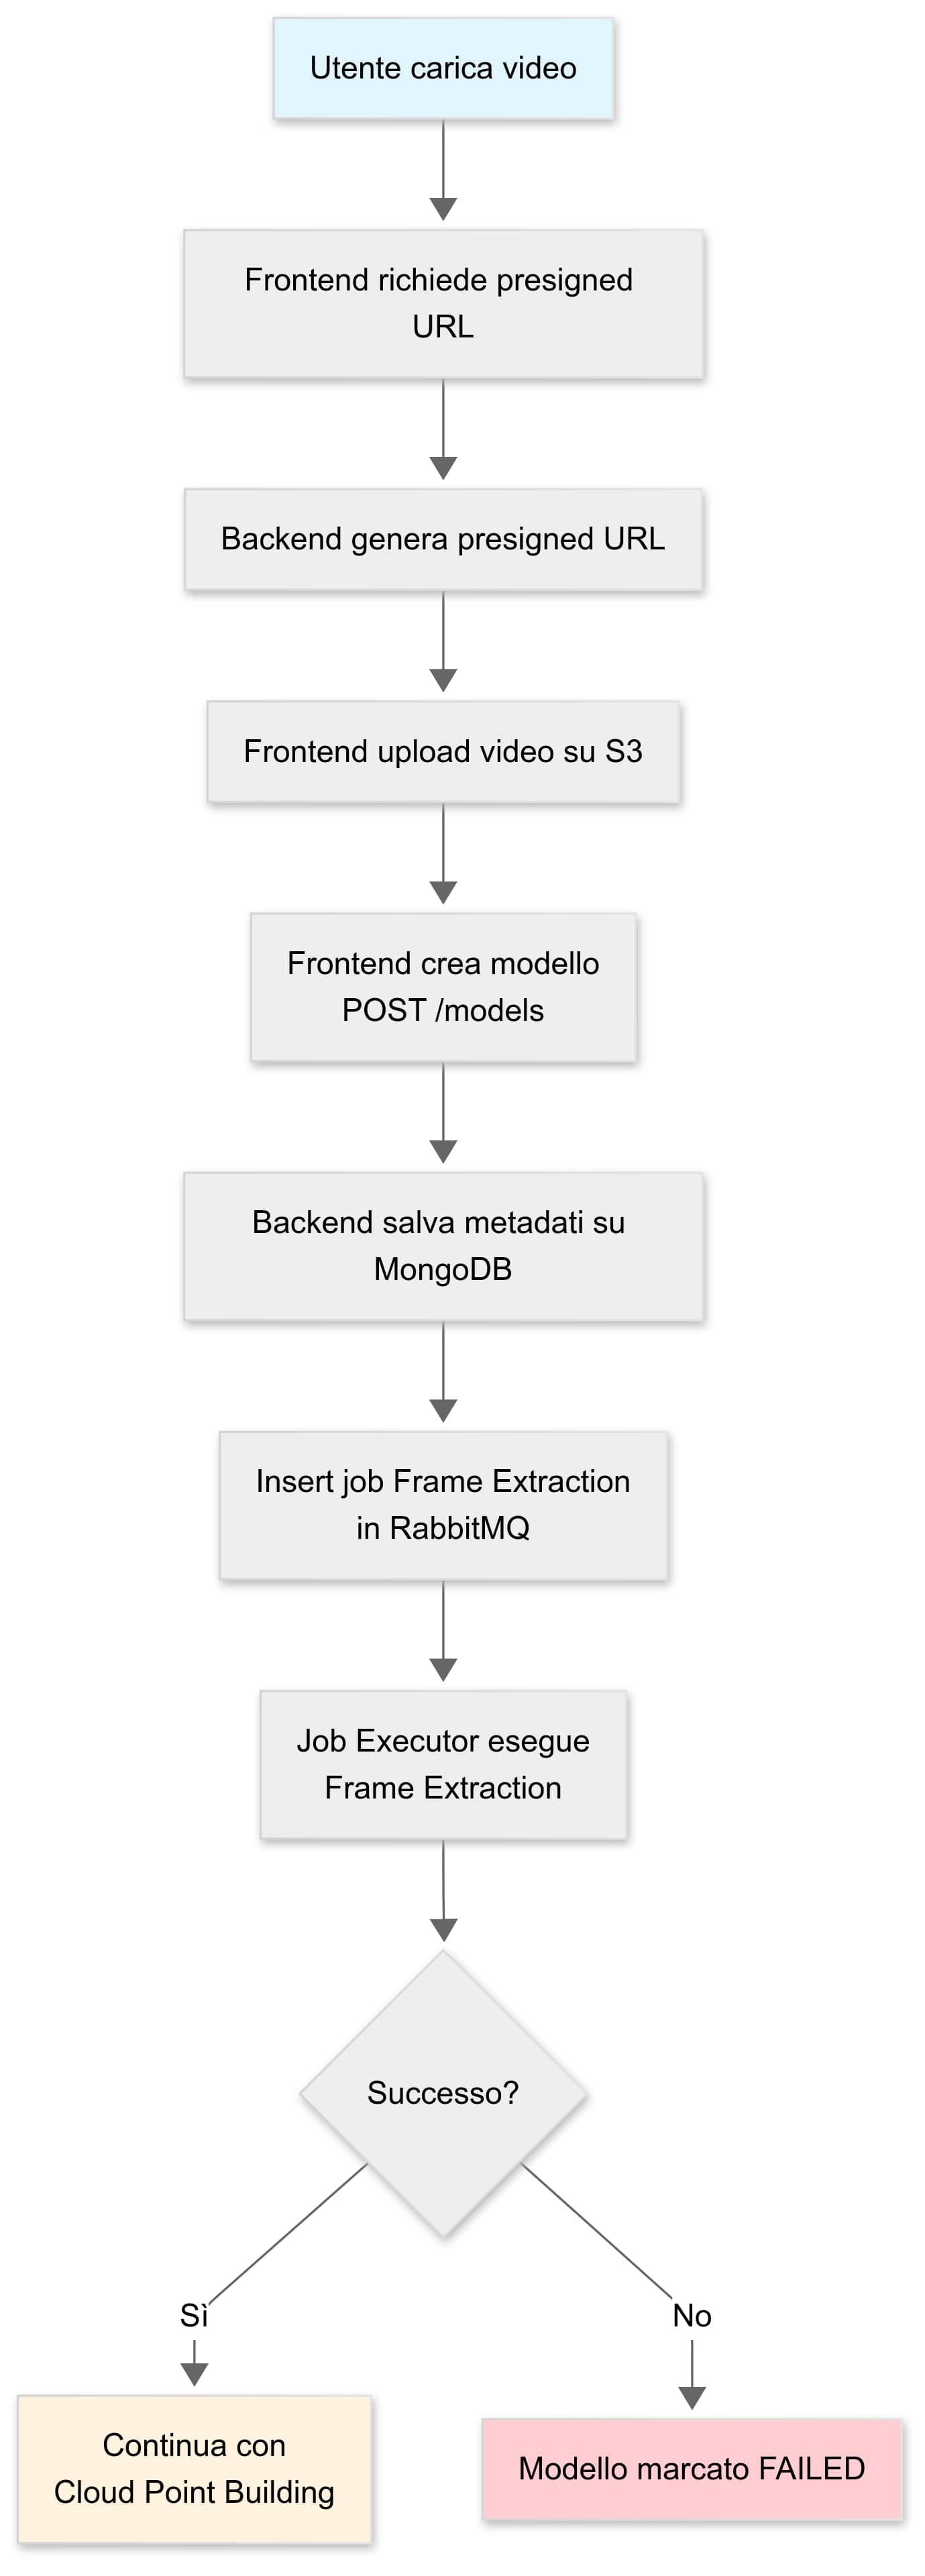
\includegraphics{images/upload_preparazione.jpg}
}
\vspace*{-0.5cm} % Riduci spazio tra figura e didascalia
\caption{Architettura dei componenti del sistema (upload e preprocessing video)}
\label{fig:component_architecture1}
\end{figure}

\begin{figure}[htbp]
\centering
\vspace*{-3cm} % Riduci spazio sopra la figura
\adjustbox{width=0.5\textwidth,center,keepaspectratio}{
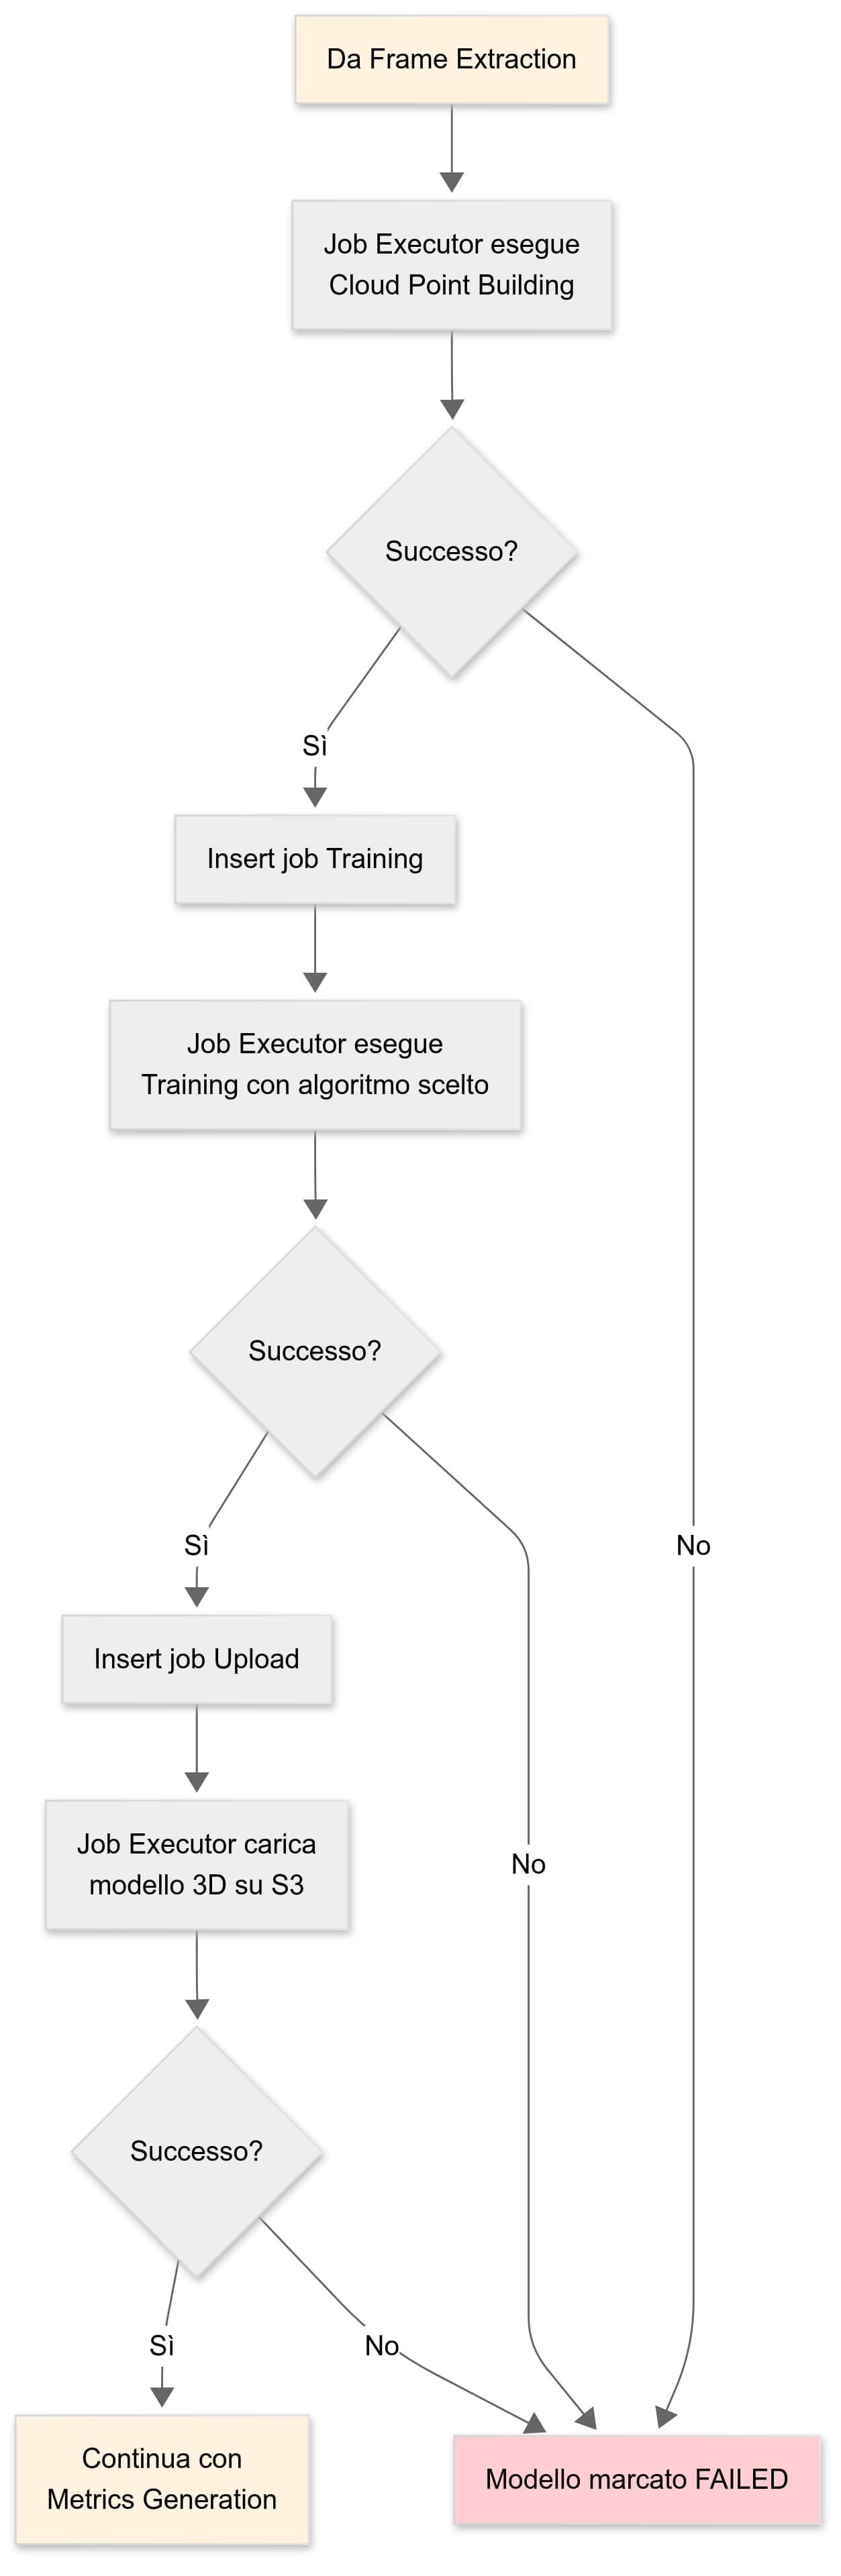
\includegraphics{images/elaborazione_training.jpg}
}
\vspace*{-0.5cm} % Riduci spazio tra figura e didascalia
\caption{Architettura dei componenti del sistema (elaborazione e training)}
\label{fig:component_architecture2}
\end{figure}

\begin{figure}[htbp]
\centering
\vspace*{-1cm} % Riduci spazio sopra la figura
\adjustbox{width=0.6\textwidth,center,keepaspectratio}{
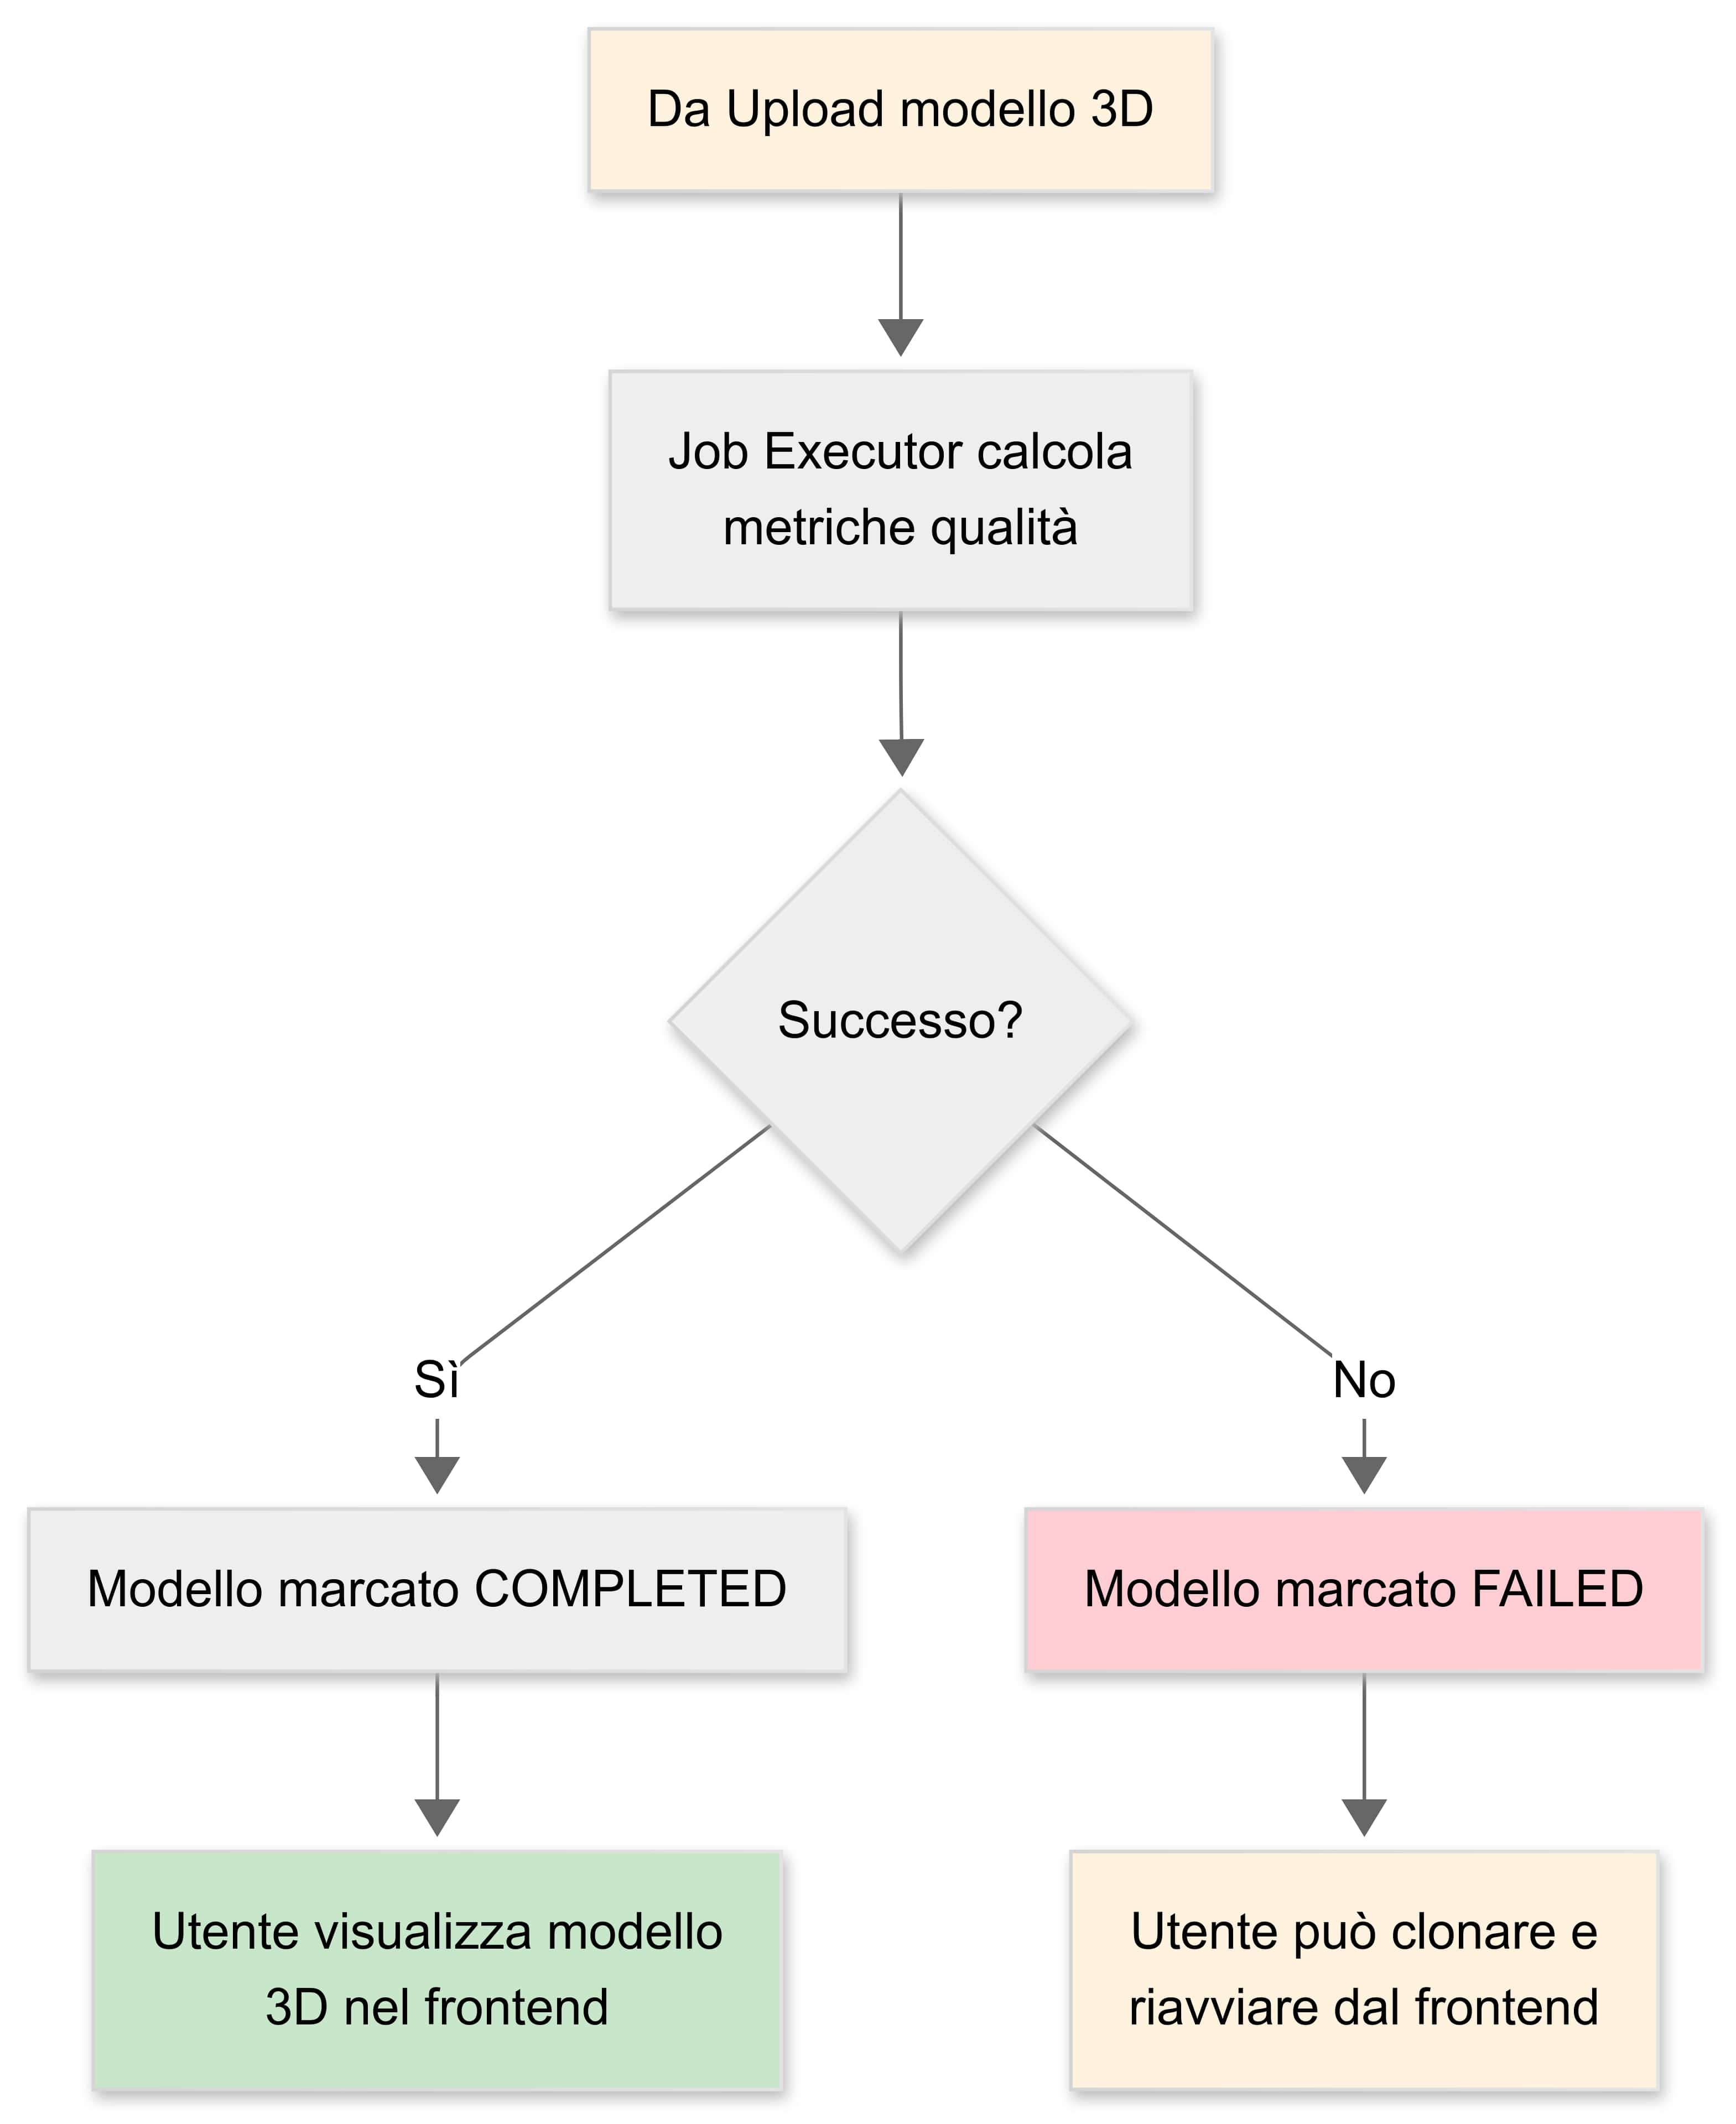
\includegraphics{images/finalizzazione.jpg}
}
\vspace*{-0.5cm} % Riduci spazio tra figura e didascalia
\caption{Architettura dei componenti del sistema (finalizzazione)}
\label{fig:component_architecture}
\end{figure}
